\section{Architectural Views}

\subsection{Context View}

\subsubsection{Stakeholders' Uses of This View}

In this view, system context is provided, with the actors and other systems related to it in a general manner. Website maintainers and Data collections of Afetbilgi will be the ones that primarily use this view to better understand how the different actors interact in the working of this website and the relationship that the system has with other external entities like the AWS components, Maps API component, and so on.

\subsubsection{Context Diagram}

% Checked in grammarly
\afetbilgi \cite{afetbilgi} is not part of a more extensive system. It is a standalone and open-source efforted website to verify critical information in the fight against the 6 February 2023 Pazarcik Earthquake and deliver it to disaster victims and those who want to help in an understandable, concise manner in multiple languages.

This information is presented in either the form of legible tables with third-party governmental and private links or an interactable method via a map view interface. If deemed necessary, admin and maintainers can make changes to display newly created or edited data and upload it to the system upon any complaints or suggestions they may get on their contact details.

\begin{figure}[H]
  \centering
  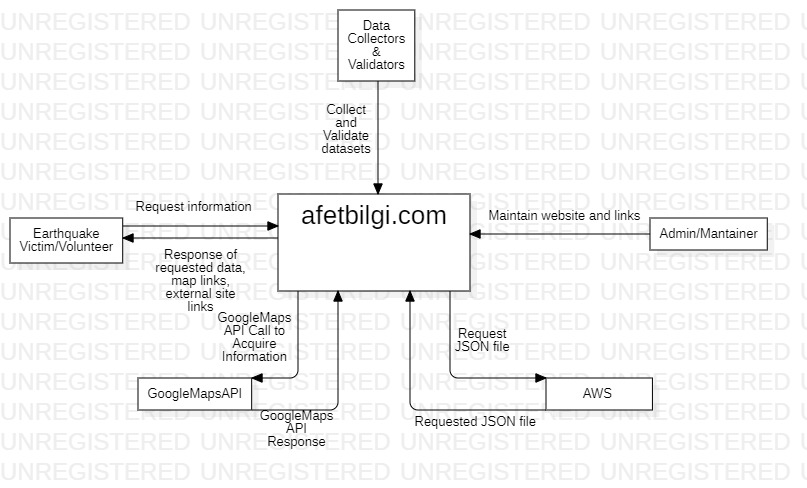
\includegraphics[width=\linewidth]{img/context-diagram.jpg}
  \caption{Context Diagram for \afetbilgi}
\end{figure}

The \afetbilgi\ consists of a combination of small physical and software parts. With the help of interfaces, these parts communicate among themselves and with the user.

\subsubsection{External Interfaces}

In this section, the external interfaces of the \afetbilgi will be provided, as well as their operations and relationships.

\begin{figure}[H]
  \centering
  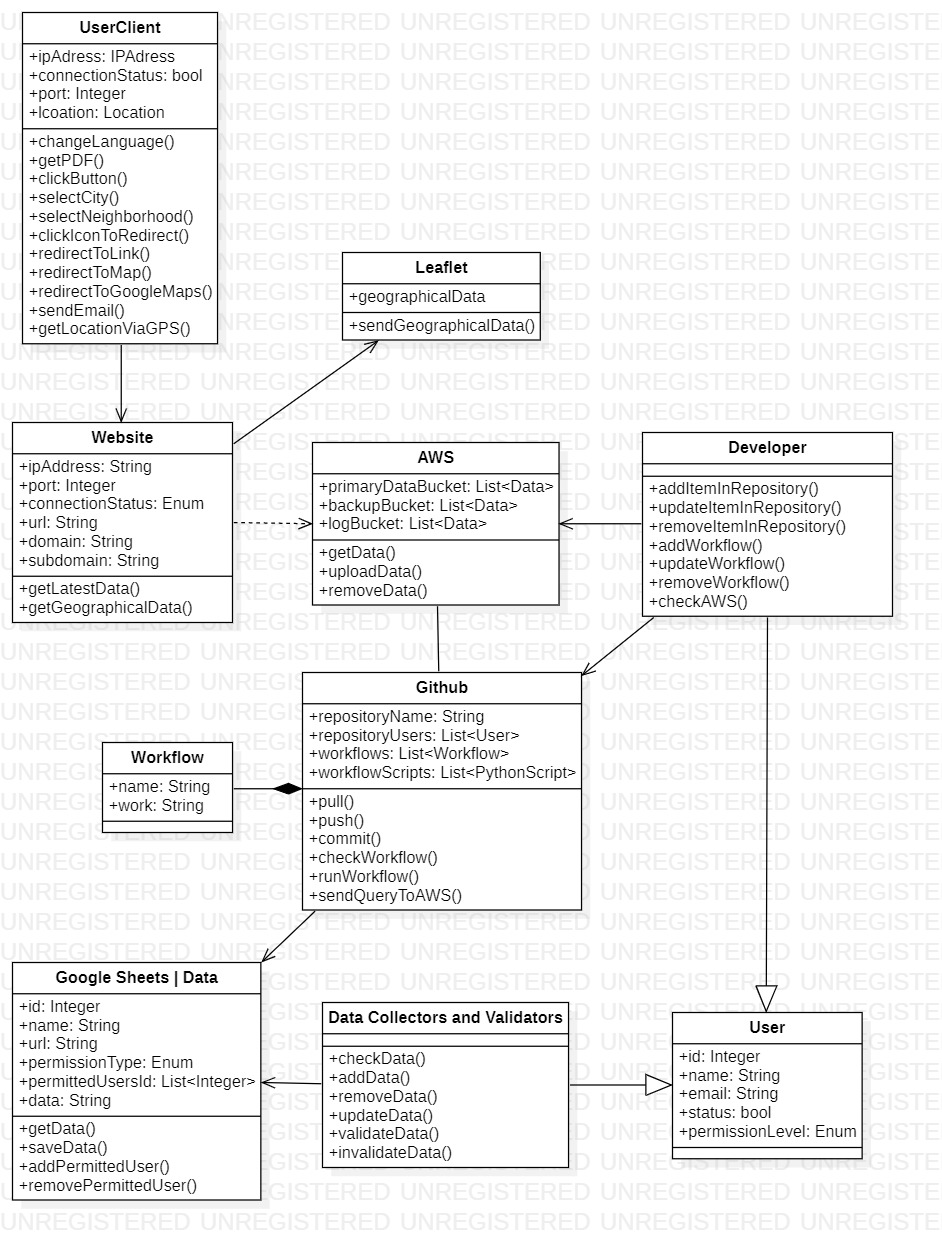
\includegraphics[width=\linewidth]{img/external-interfaces-diagram.jpg}
  \caption{External Interfaces}
\end{figure}

As it can be observed from Figure \addnumbertofigure{0}, \afetbilgi has multiple external interfaces. UserClient, Website, Leafler, AWS, Developer, Google Sheets for data, Data Collectors and Validators are external interfaces of the system. Github Repository for the \afetbilgi may also ve considered an external interface since it is generally responsible for sustainability of the system. The operations given in the diagram can be summarized as follows:

\begin{itemize}
  \item The Data Collectors and Validators collect data and validate it. After validation, data is added into a specificied data sheet in Google Sheets.
  \item Google Sheets mainly store the data. The data is divided into several files in Google Sheets. These sheets can be accessible for data collectors and validators.
  \item GitHub Repository is used storing the source code. Additionally, the GitHub workflows of the repository check, maintain and update the website in regular basis by executing the workflows in a determined period.
  \subitem Some workflows use the scripts in the repository to access sheets to get the recent data and create new updated \texttt{latest.json} and \texttt{schema.json} files. After completing the creation of these files, they are uploaded to Amazon Web Services (AWS). These workflows can be managed and updated by the developer.
  \item Leaflet is used for the map of the afetbilgi. There is additional subdomain, whose link is \href{https://maps.afetbilgi.com}{maps.afetbilgi.com} for the complete map.
  \item UserClient initiate the connection with the website. It has some attributes that are provided to website and functionalities to control the website.
\end{itemize}

\subsubsection{Interaction Scenarios}

Two different interaction scenarios are provided:

\begin{figure}[H]
  \centering
  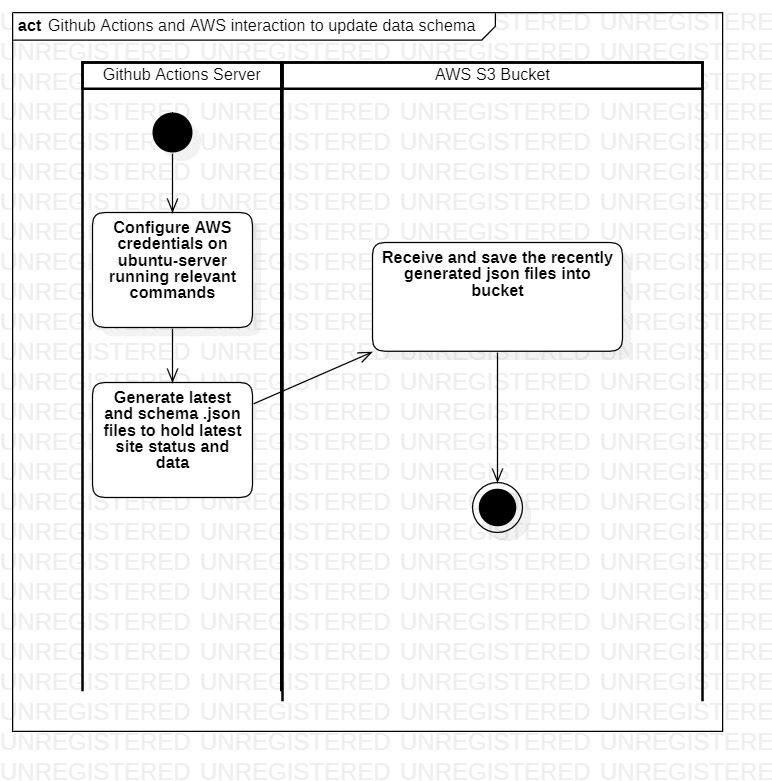
\includegraphics[width=\linewidth]{img/activity-diagram-1.jpg}
  \caption{Activity Diagram | GitHub Actions and AWS Interaction to Update Data Schema}
\end{figure}

\begin{figure}[H]
  \centering
  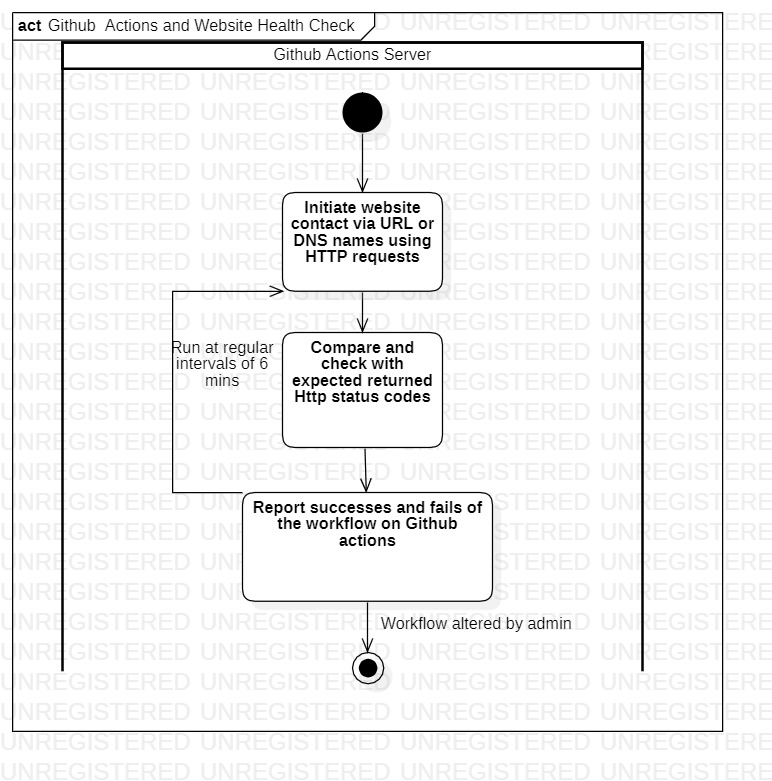
\includegraphics[width=\linewidth]{img/activity-diagram-2.jpg}
  \caption{Activity Diagram | GitHub Actions and Website Health Check}
\end{figure}

\subsection{Functional View}

\subsubsection{Stakeholders' Uses of This View}

This view depicts the different components of the system and their interaction, including the internal interfaces. This is extremely important for the stakeholders as it gives information about the system's functionalities and the integral properties, it also gives way for other viewpoints and diagrams. As such victims and volunteers wont find this useful but website maintainers along with Data collectors would deeply appreciate this view to understand internal components and perhaps come up with ways to improve it.

\subsubsection{Component Diagram}

\begin{figure}[H]
  \centering
  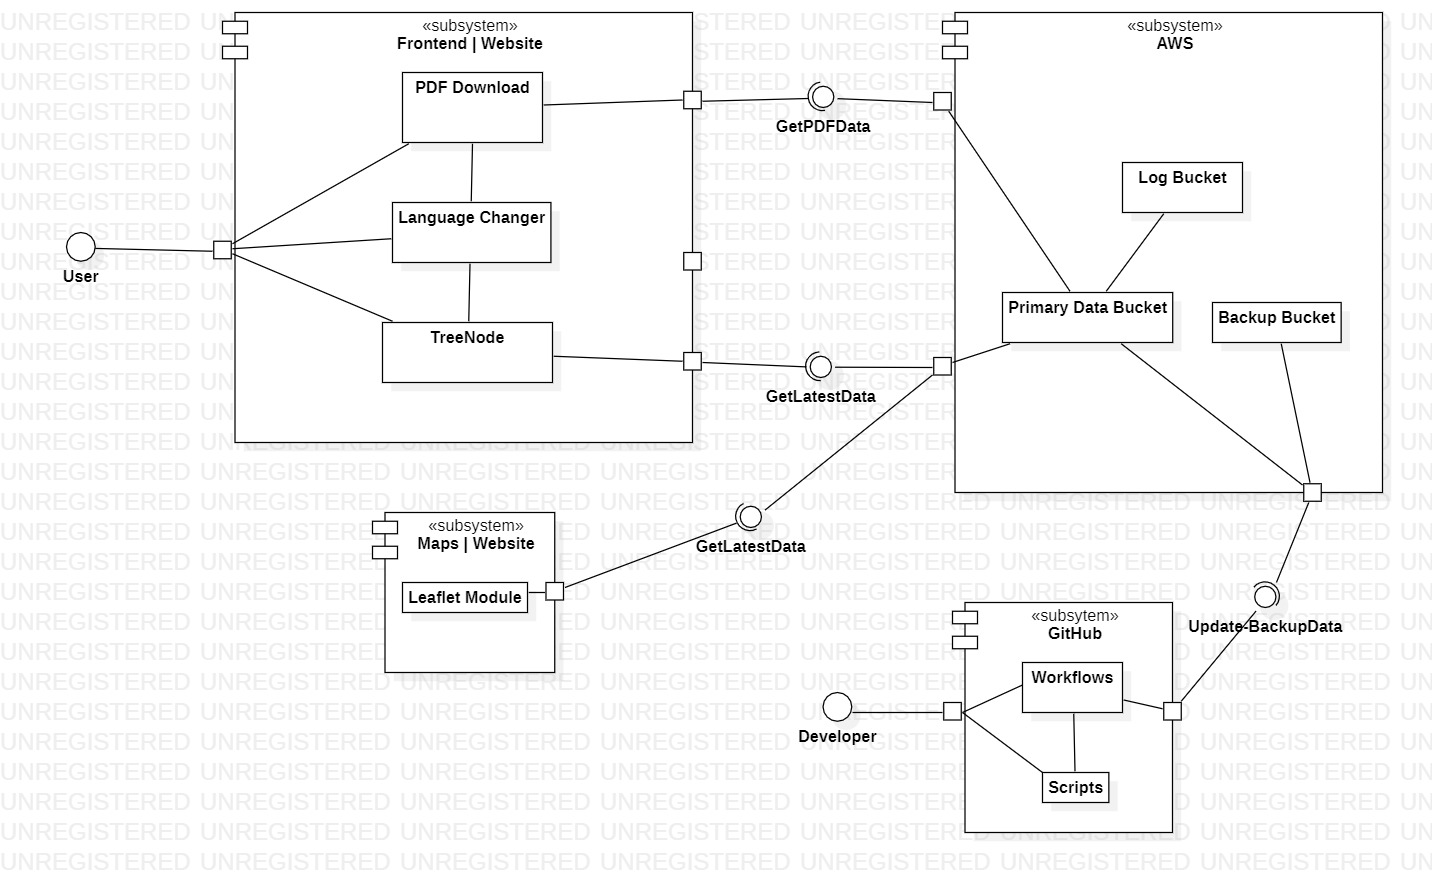
\includegraphics[width=\linewidth]{img/component-diagram.jpg}
  \caption{Component Diagram}
\end{figure}

Our system have four subsytems. Two of them subsystem is website subsytems.
\begin{itemize}
  \item The website has two different subsystems which are the frontend, the main website, and the map, providing the map feature.
  \item The map subsystem use leaflet to show the data more effectively on the map.
  \item The frontend subsystem is divided into components to handle different request from the user.
  \subitem It includes PDF component to get the PDF version of the website to use and distribute the website in offline mode. The PDF files are generated by workflows and stored in AWS.
  \subitem This subsystem also has language changer to update the language setting of the website so that user can access the website in different language to use.
  \subitem TreeNode is the main display component. It parse the data after getting the latest available data, \texttt{latest.json}, from the AWS.
  \item AWS is mainly used to \texttt{latest.json} (data), \texttt{schema.json} (schema of the \texttt{latest.json}) and PDFs.
  \item Github subsystem includes scripts and workflows. Scripts are generally written in python and used by the workflows. Workflows are responsible for checking, maintaining and updating the website in regular basis.
\end{itemize}

\subsubsection{Internal Interfaces}

\begin{figure}[H]
  \centering
  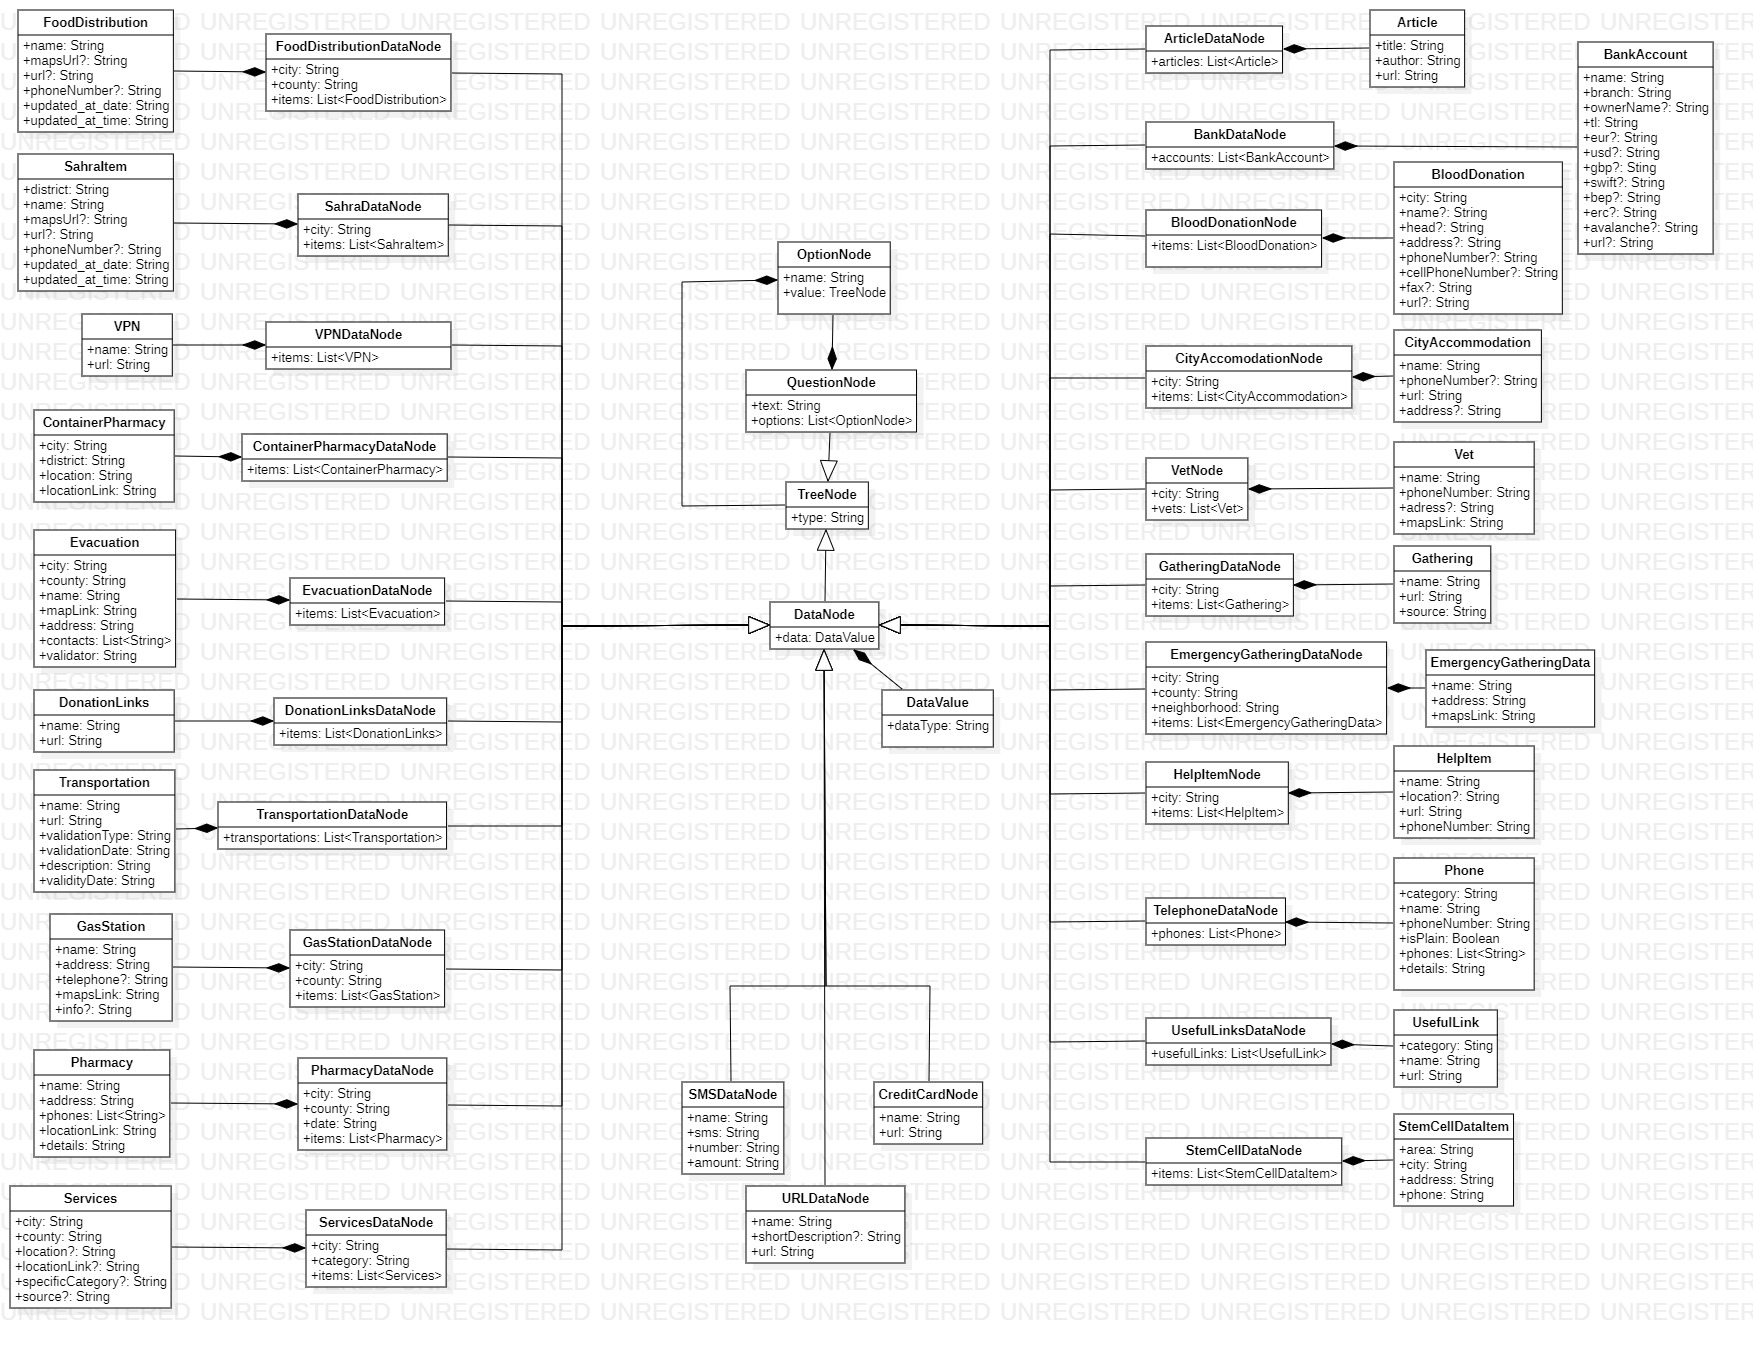
\includegraphics[width=\linewidth]{img/internal-interfaces-diagram.jpg}
  \caption{Internal Interfaces}
\end{figure}

There is no internal dynamism between interfaces. The internal interfaces are just the data interfaces to provide structured information for frontend code so that frontend code can parse the information correctly and fastly.

The main data is stored in the AWS in \texttt{latest.json} and retrieved from AWS so that the frontend code parses the data.

\subsubsection{Interaction Patterns}

\begin{figure}[H]
  \centering
  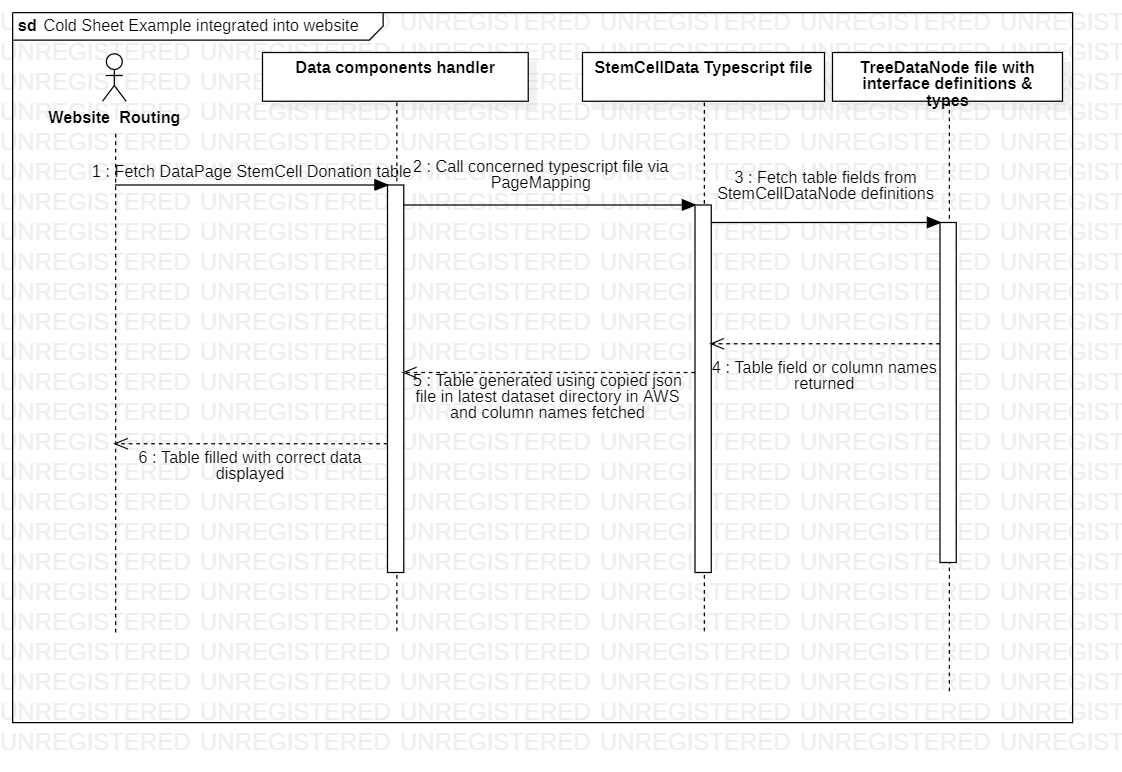
\includegraphics[width=\linewidth]{img/sequence-diagram-1.jpg}
  \caption{Sequence Diagram | Cold Sheet Example Integrated Into Website}
\end{figure}

\begin{figure}[H]
  \centering
  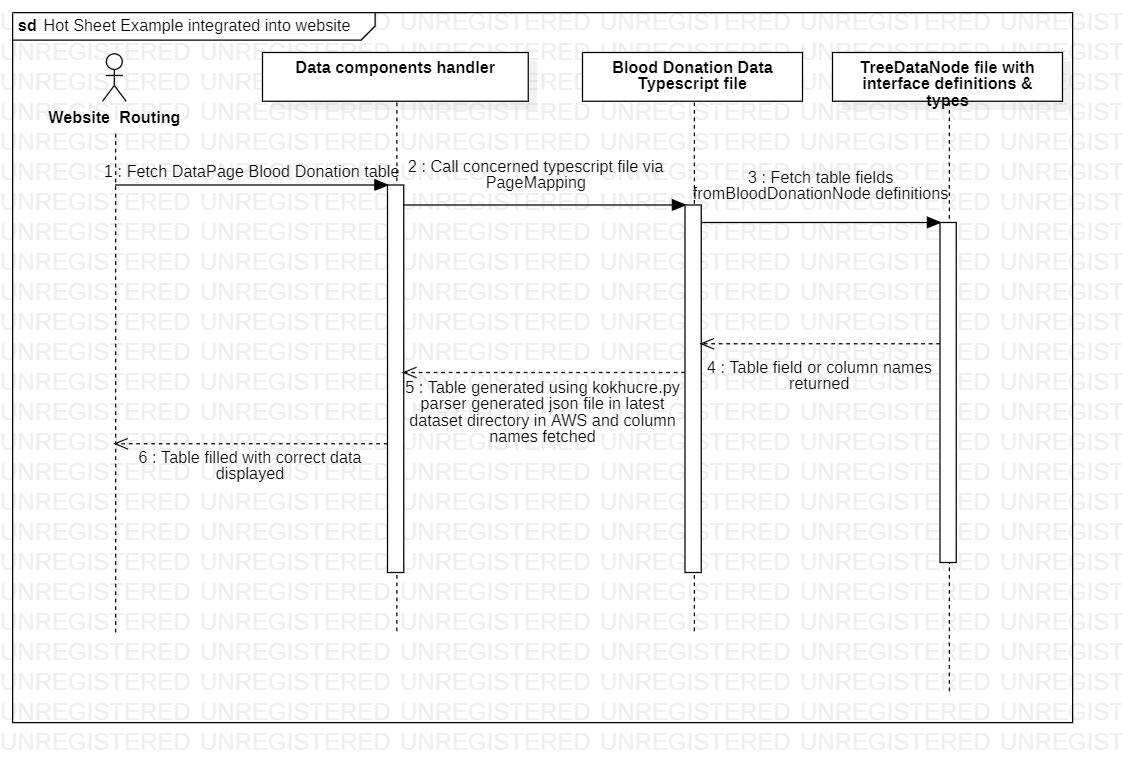
\includegraphics[width=\linewidth]{img/sequence-diagram-2.jpg}
  \caption{Sequence Diagram | Hot Sheet Example Integrated Into Website}
\end{figure}

\begin{figure}[H]
  \centering
  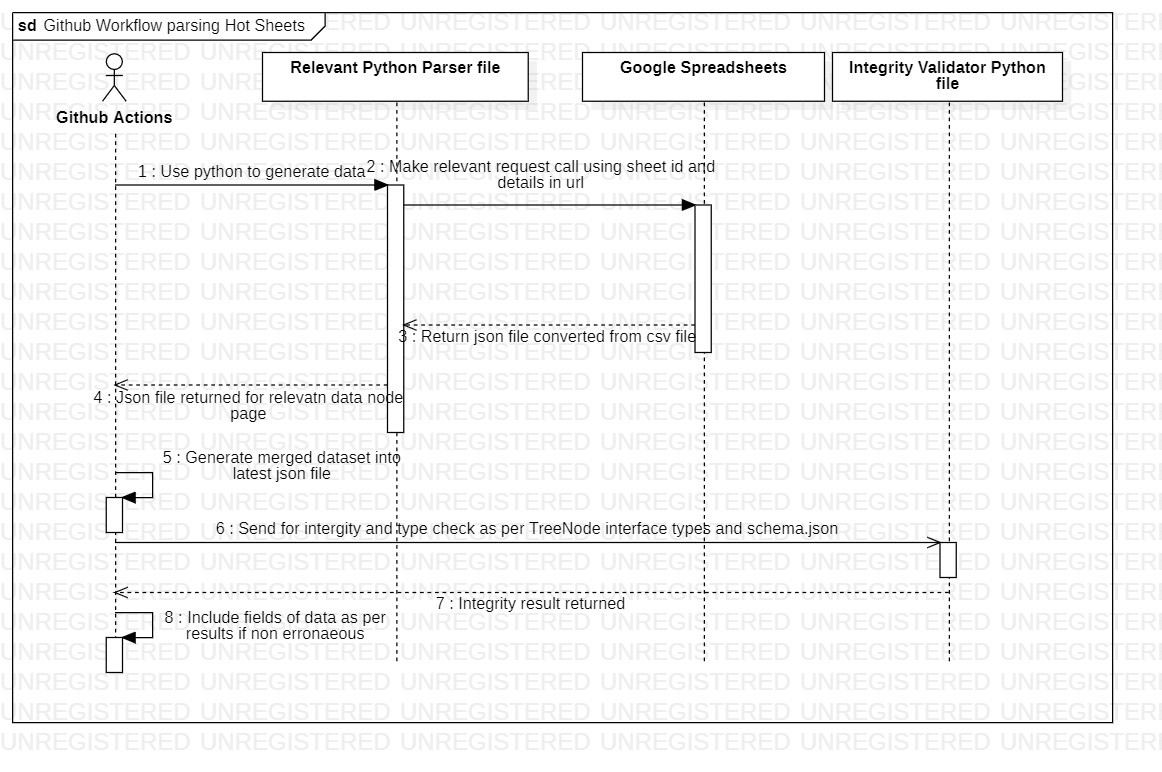
\includegraphics[width=\linewidth]{img/sequence-diagram-3.jpg}
  \caption{Sequence Diagram | GitHub Workflow Parsing Hot Sheets}
\end{figure}

\subsection{Information View}

\subsubsection{Stakeholders' Uses of This View}

This view concerns the variables and the data used and stored in this system during use as per Rozanski's explanations. While this open-source, static and nondynamic website doesn't employ a database infrastructure backend like mySQL, stakeholders such as website maintainers along with data maintainers/validators would again appreciate to know which data pages and nodes are being exchanged and whether any unreliable information is being or has been uploaded to the website assets and datasheets.

\subsubsection{Database Class Diagram}

\begin{figure}[H]
  \centering
  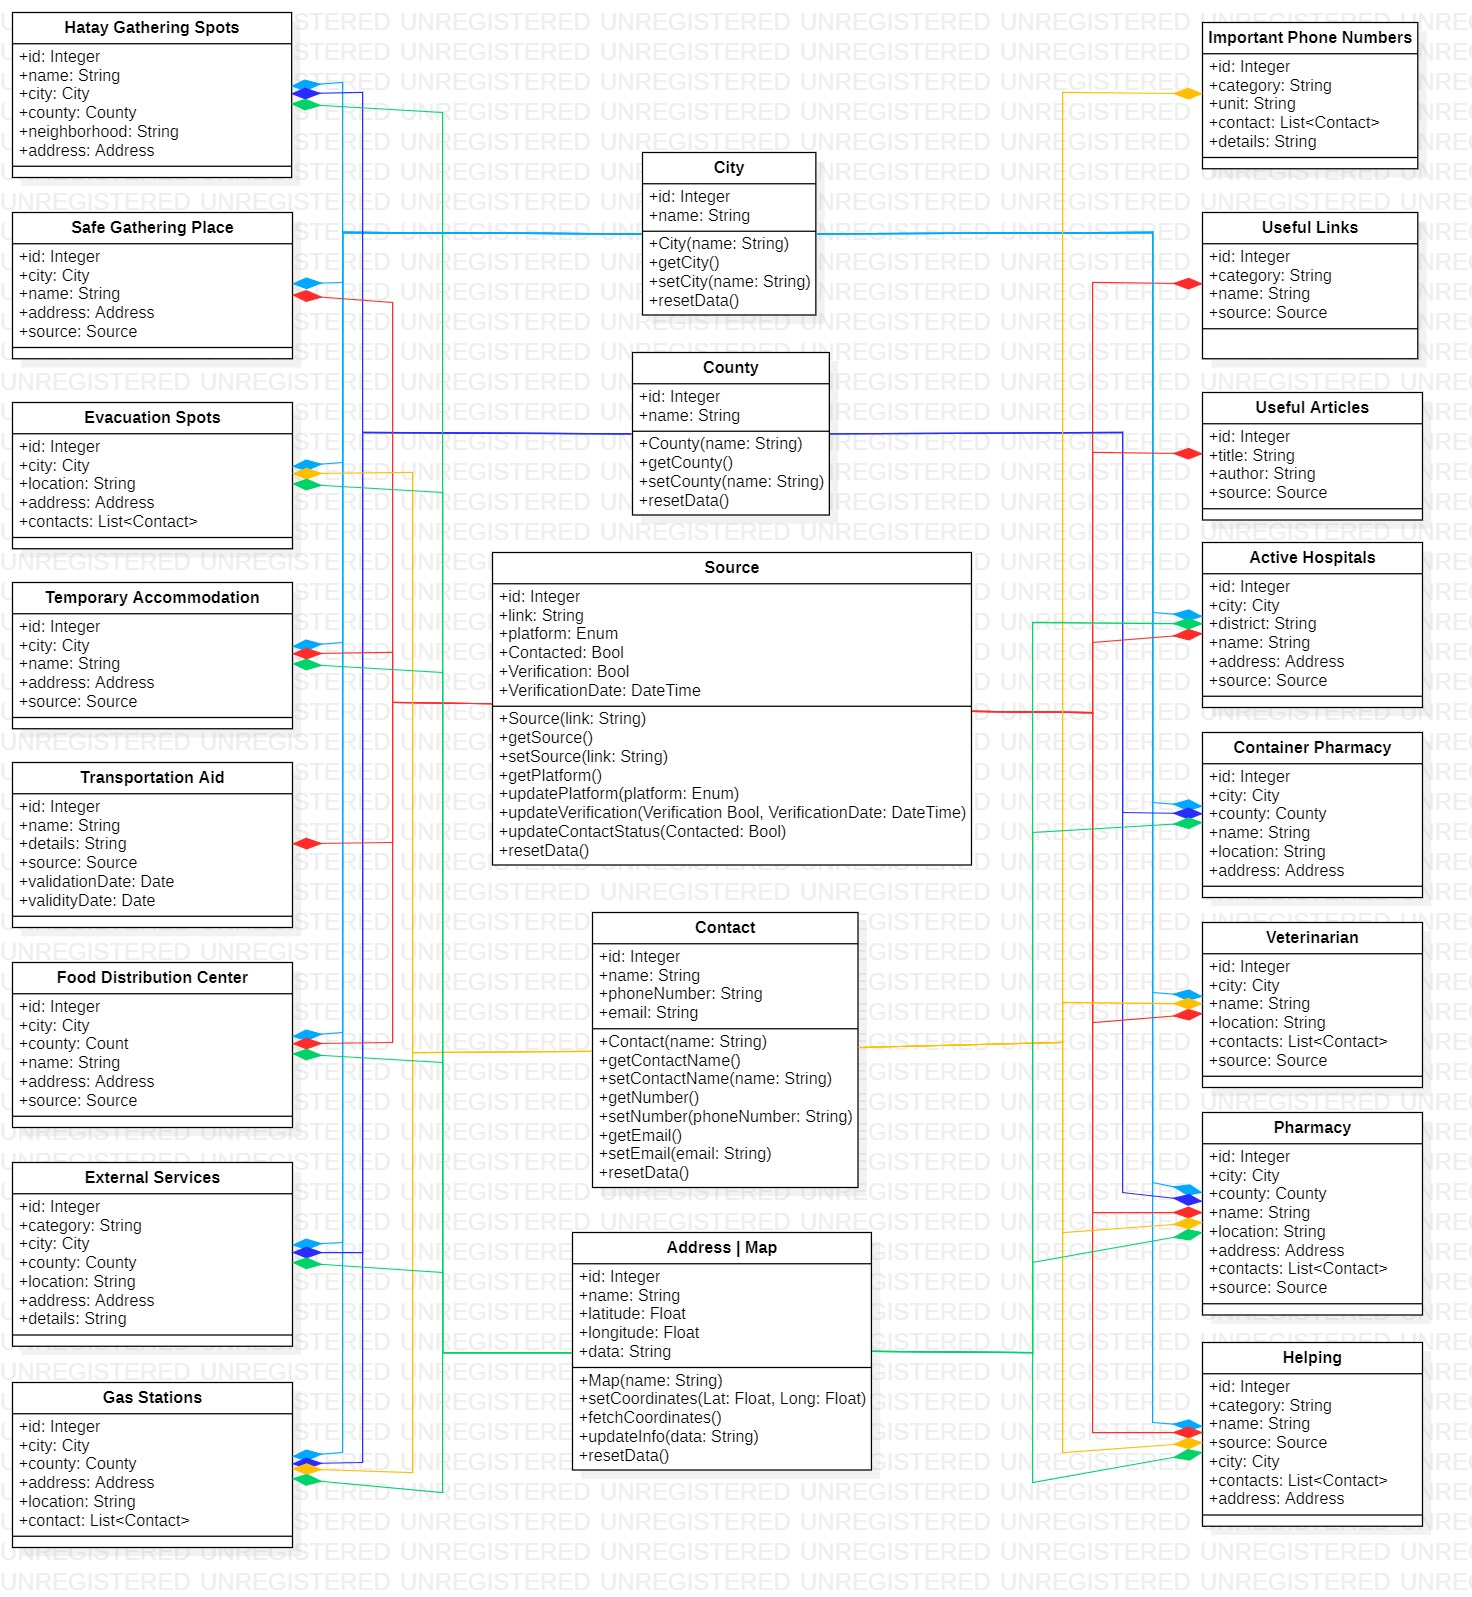
\includegraphics[width=\linewidth]{img/database-class-diagram.jpg}
  \caption{Database Class Diagram}
\end{figure}

\subsubsection{Operations on Data}

\begin{table}[H]
  \centering
  \begin{tabular}{|l|l|}
    \hline
    Operation & CRUD Operation \\ \hline
    City::City & Create: City Profile with name \\
               & Read: \\
               & Update: \\
               & Delete: \\ \hline
    City:: getCity() & Create: \\
                     & Read: City for selection \\
                     & Update: \\
                     & Delete: \\ \hline
  \end{tabular}
  \caption{CRUD Operations on Data}
\end{table}

\subsection{Deployment View}

\subsubsection{Stakeholders' Uses of This View}

Rozanski's document explained the deployment view as the environment in which the system in running(inclusive of hardware/external server elements). As such in this project's case, the website maintainers/admins would be the ones to appreciate a basic amount of knowledge from the deployment diagram below such as the basic relations such as how to run parser script files and set up hot/cold sheets which are regularly updated to latest.json via the AWS s3 bucket. On the other hand, future/long term site maintainers would be wanting to take the analysis of the deployment diagram even further to develop and focus on individual parts comprising the components such as improving coldsheets' static json files that can be secured perhaps a bit more before being merged to formed recent latest.json files.

\subsubsection{Deployment Diagram}

\begin{figure}[H]
  \centering
  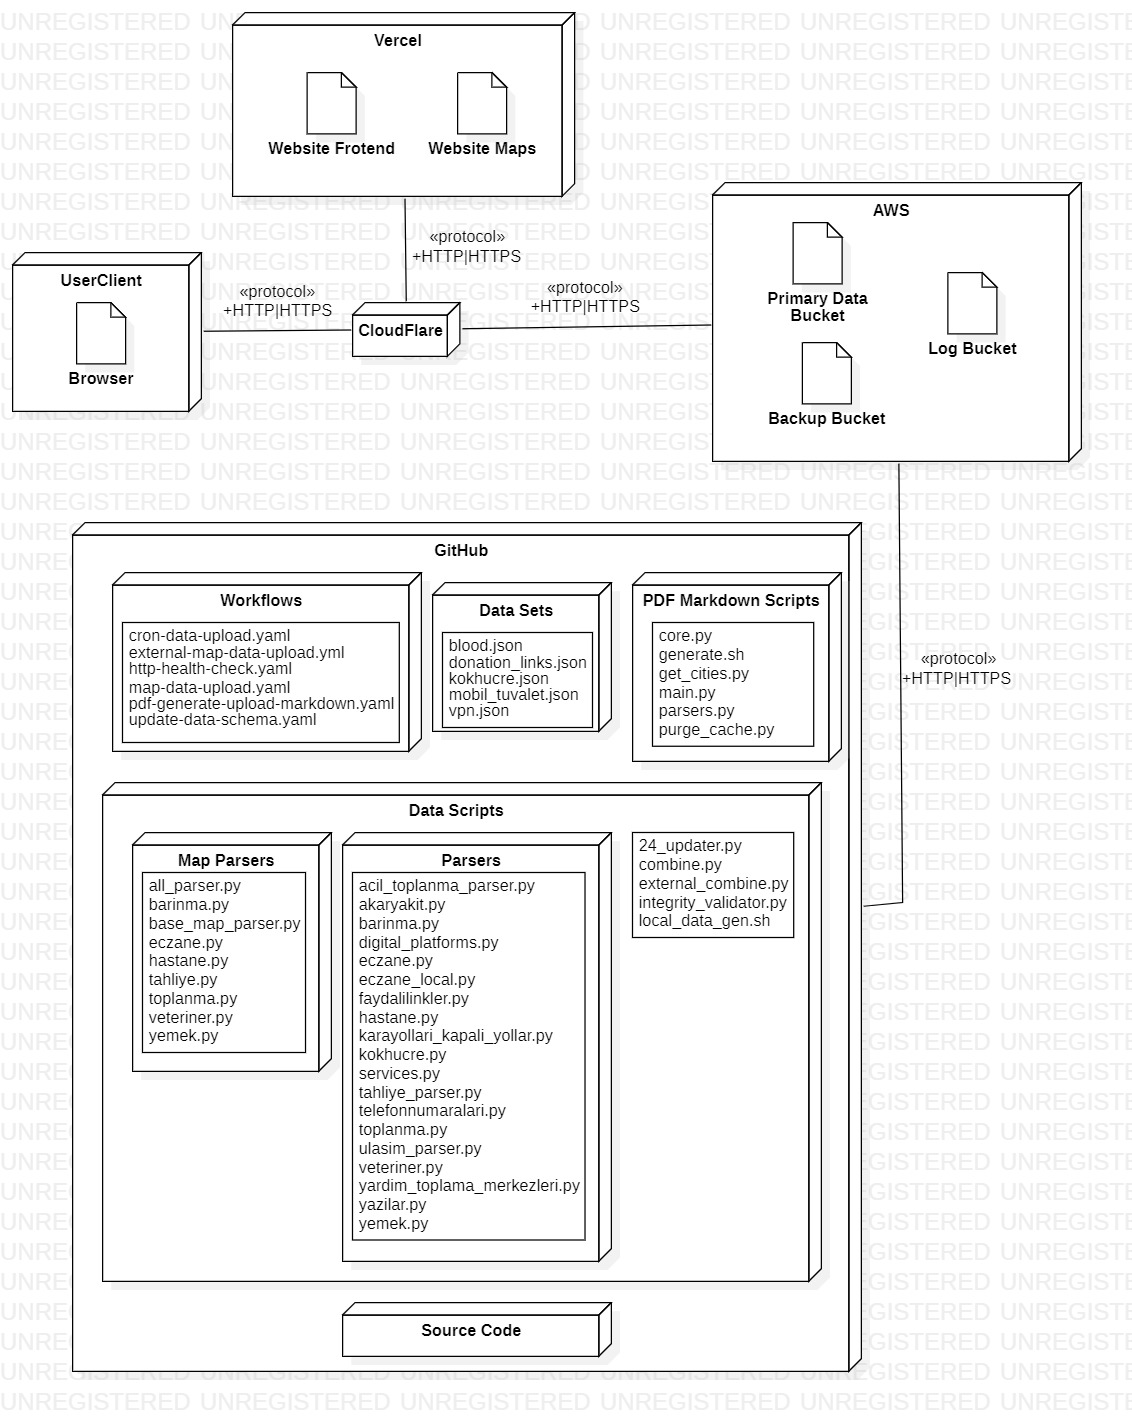
\includegraphics[width=\linewidth]{img/deployment-diagram.jpg}
  \caption{Deployment Diagram}
\end{figure}

In our deployment diagram viewpoint, we show the deployment environment of the \afetbilgi.
\begin{itemize}
  \item User should use a javascript supported browser to access the website.
  \item Requests are met by CloudFlare and CloudFlare maps the related request. CloudFlare also gives supports for general protection such as using HTTPS, TLS and DDoS protection as well as the general protection.
  \item Vercel contains the website with both frontend and maps.
  \item AWS includes the primary data which is \texttt{latest.json} and other data. It also stores the bakcups and logs.
  \item GitHub provides source code and workflows. Workflow of GitHub checks, maintains and updates the data and the website. These workflows uses scripts to get the latest and stored data data and combine them to upload to AWS. Also, PDFs are generated and upload to AWS.
  \item Google Sheets store the data updated by data collectors and validators.
\end{itemize}

\subsection{Design Rationale}

The whole afetbilgi website system is based on the premise and primary rationale that it's an open source, verified non-profit website, which aims to convey quick information to victims and volunteers alike without any user registration/related overhead requiring unnecessary time expenditure. It's based on a website with plain buttons and hierarchical routing leading to relevant datasheets as per need. All the views consisting of context, functional, information and deployment build on this.

In the context view, the basic setup is explained in the context diagram showing how maintainers have set up the website of afetbilgi to be used by victims and volunteers alike. The external interface diagram further improves on this showing how the data validators used external services like Google Datasheets to fetch recent data, as well as AWS to use assimilated data from latest.json. On the other hand site maintainers and developers have also used Github Actions' CI/CD workflows to continuously update the website and check its data health regularly from the AWS S3 bucket where it's hosted and its DNS assignments are covered by Cloudflare. 

In the functional view, we see the internal interfaces interact in a modern modular setup(as per object programming's interface and extension principles). On the computation component sides, it's explained how the website health is checked regularly using the workflow actions from Github on ubuntu environments with backups of data and the last health website saved to buckets in AWS, while on the internal interface we learn of modularized entities like TreeNode interfaces which strictly check how new data pages are added and how their typing match to the node description as per their specification. As the website is static and every such Data node(each having own webpage on the afetbilgi website) doesn't really interact with any other interface yet the sequence diagrams great demonstrate how new data(hot/cold) is added and conformed to the node specifications while the Workflows assimilate and eventually upload then to AWS as latest.json files(types checked and saved via schema.json too). 

Information View reinforces the stand alone concept of this project with no backend databases and no area to upload any private information such user info/credit card detail,etc . The site data validators and maintainers  are the main stakeholders to appreciate this section, knowing which variables transmit and exchange within which interfaces as shown on the Database Class diagram. There are no explicit SQL classes or tables yet there is some sort of validation/role allotment needed for a user to be allowed to update data on the website. All the tables/datasheets have common elements of City, Source, Location and Map components present. The CRUD operations' table helps in having a basic summary of the presented data-altering options from the Database Class Diagram without too much technicalities. 

Lastly, the Deployment View again explains the project repository and the modular nature of this project, with the files clearly set out. Over here, we see the dependent nature of this project with other external entities to upload data to or interact with such as the AWS bucket components and exchanging latest.json files with them along with type conformations in schema.json. Parser python files are run via external Github actions' ubuntu server to run and assimilate hot data sheets after fetching from the relevant Google Datasheets while cold sheets(manually added data) are simply copied and merged.
